\documentclass[tikz,border=2pt]{standalone}
\usepackage{amsmath,amssymb}
\usepackage{tikz}
\usetikzlibrary{arrows.meta}

\begin{document}
% A stochastic process is a family of random variables indexed by time; each run of the
% experiment produces one sample path (two paths of a simple random walk are shown).
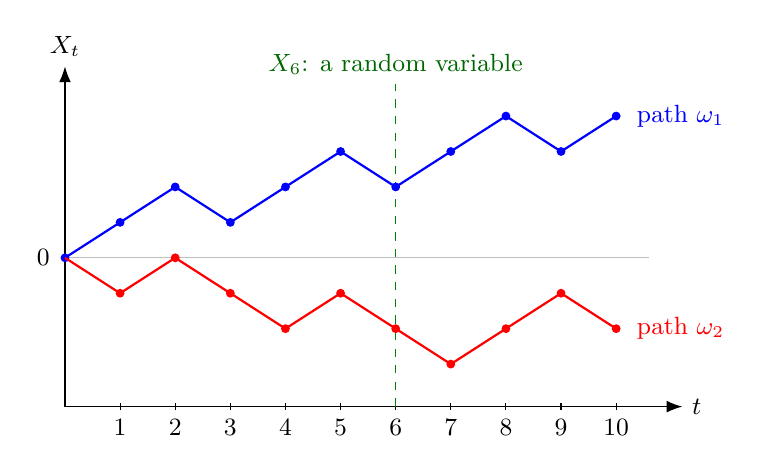
\begin{tikzpicture}[every node/.style={font=\small}, >={Latex[length=2mm]}, x=0.7cm, y=0.45cm]
	\draw[->] (0,-4.2) -- (11.2,-4.2) node[right] {$t$};
	\draw[->] (0,-4.2) -- (0,5.4) node[above] {$X_t$};
	\draw[gray!50] (0,0) -- (10.6,0);
	\node[anchor=east, font=\small] at (-0.1,0) {$0$};
	\foreach \t in {1,...,10} {\draw (\t,-4.1) -- (\t,-4.3); \node[below=1pt, font=\small] at (\t,-4.2) {\t};}
	\draw[green!50!black, dashed] (6,-4.2) -- (6,4.9);
	\draw[blue, thick] (0,0) -- (1,1) -- (2,2) -- (3,1) -- (4,2) -- (5,3) -- (6,2) -- (7,3) -- (8,4) -- (9,3) -- (10,4);
	\foreach \t/\y in {0/0,1/1,2/2,3/1,4/2,5/3,6/2,7/3,8/4,9/3,10/4} {\fill[blue] (\t,\y) circle (1.6pt);}
	\draw[red, thick] (0,0) -- (1,-1) -- (2,0) -- (3,-1) -- (4,-2) -- (5,-1) -- (6,-2) -- (7,-3) -- (8,-2) -- (9,-1) -- (10,-2);
	\foreach \t/\y in {1/-1,2/0,3/-1,4/-2,5/-1,6/-2,7/-3,8/-2,9/-1,10/-2} {\fill[red] (\t,\y) circle (1.6pt);}
	\node[green!40!black, font=\small, anchor=south] at (6,4.9) {$X_6$: a random variable};
	\node[blue, anchor=west, font=\small] at (10.2,4) {path $\omega_1$};
	\node[red, anchor=west, font=\small] at (10.2,-2) {path $\omega_2$};
	
\end{tikzpicture}
\end{document}
